\title{Overview of ESMValTool}
\date{\today}

\documentclass[12pt]{article}
\usepackage{graphicx}
\usepackage[square,comma,numbers,sort&compress]{natbib}
\usepackage[pdfauthor={Martin.Evaldsson@smhi.se},
            pdftitle={Overview of ESMValTool},
            pdfkeywords={EMBRACE, work package 4},
            pdfsubject={EMBRACE WP 4 visualisation tool}]{hyperref}
\usepackage[hyphenbreaks]{breakurl}
\usepackage[all]{hypcap}
\usepackage{url}
\usepackage{varioref}
\usepackage{multirow}
\usepackage{rotating}
\usepackage{fancyvrb}
\usepackage{color}
\usepackage{amsmath}
\usepackage{titlesec}

\definecolor{dark-red}{rgb}{0.4,0.15,0.15}
\definecolor{dark-blue}{rgb}{0.15,0.15,0.4}
\definecolor{medium-blue}{rgb}{0,0,0.5}
\hypersetup{
        colorlinks, linkcolor={dark-red},
        citecolor={dark-blue}, urlcolor={medium-blue}
}

\newenvironment{myverb}{\footnotesize\begin{Verbatim}[frame=single, fontsize=\footnotesize]}{\end{Verbatim}}
%% Define a new 'leo' style for the package that will use a smaller font.
\makeatletter
\def\url@leostyle{%
  \@ifundefined{selectfont}{\def\UrlFont{\sf}}{\def\UrlFont{\small\ttfamily}}}
\makeatother
%% Now actually use the newly defined style.
\urlstyle{leo}

\newcommand{\docref}[1]{`\emph{#1}'}
\newcommand{\xmltag}[1]{\texttt{$<$#1$>$}}

\setcounter{secnumdepth}{5}

\begin{document}
\maketitle

%%%%%%%%%%%%%%%%%%%%%%%%%%%%%%%%%%%
% 
% INTRODUCTION
% 
%%%%%%%%%%%%%%%%%%%%%%%%%%%%%%%%%%%
\phantomsection
\section{Introduction}\label{section:introduction}
The ESMValTool is a software package used to compare and visualize
climate data sets. The tool reads climate data from CMIP5 compliant
netCDF files and generates output in postscript, pdf, png or
netCDF-files. This document gives a practical overview of the tool;
describing its background, the project workflow, the control flow of
the tool and basic operations such as configuring it to produce a
certain plot/variable, how to add new plot scripts/variables. Specific
issues are further explained in  the ESMValTool
\docref{doc/reference.pdf}. For a more ``hands-on'' approach, see the
\docref{doc/toy-diagnostics-tutorial.pdf}. The tool is directly built
upon the Chemistry-Climate-eValuation Tool\cite{CCMVal-main:2012}
(CCMVal Tool). For an in-depth technical discussion on the purpose and
possibilities with ESMValTool, please see the corresponding discussion
for CCMVal\cite{CCMVal-main:2012}. 

\paragraph*{Outline}
The remainder of this document is organized as follows.
Section~\ref{section:prerequisites} lists the ESMValTool
prerequisites, section~\ref{section:project_workflow} project
workflow, section~\ref{section:overall_structure} describes the
overall structure of the tool, section~\ref{section:config-files}
details the configuration files used by the ESMValTool,
section~\ref{section:plottingExamples} works through a number of
examples. Finally, section~\ref{section:MyDiag} describes the template
that can be used as a toy diagnostic for becoming familiar with the
ESMValTool structure.
% ############ END OF INTRODUCTION #################


%%%%%%%%%%%%%%%%%%%%%%%%%%%%%%%%%%%
% 
% ESMVAL PREREQUISITES
% 
%%%%%%%%%%%%%%%%%%%%%%%%%%%%%%%%%%%
\phantomsection
\section{ESMVal prerequisites}\label{section:prerequisites}
The ESMValTool requirements are, 
\begin{itemize}
\item{\textcolor{red}{compulsory:}} Python 2.x installation (versions
3.x will not work)

\item{\textcolor{red}{compulsory:}} NCAR Command Language
(NCL)\cite{ncar-ncl-homepage} version 6.1 or higher. Google ``install
ncl'' to find the NCAR page describing how to download and install NCL
locally

\item{\textcolor{red}{compulsory:}} CMIP5-style\cite{pcmdi-cmip5}
netCDF data sets available on the file system. In practice,
``CMIP5-style'' means that some core netCDF attributes are required to
comply with the CF-metadata conventions\cite{pcmdi-cf-conventions}
and, to work work out of the box, the netCDF input file names should
follow the CMIP5-naming convention\cite{DRS-document:2010}. Note that
the tool can be configured to accept non-CMIP5 filenames and to
rewrite non-CF compliant input files on the fly, this is described in
the \docref{doc/reference.pdf}-file.

\item{\textcolor{green}{optional:}} The R scripting
language\cite{R-language-ref:2013} version 2.14 or later (older
version may work). R is only needed if the R-based plot scripts are
used for output. These plot scripts does in turn use the following
R-packages, 
\begin{itemize}
\item ncdf4
\item fields
\item maps
\item MASS
\item chron
\end{itemize}

\end{itemize}

% ############ END ESMVAL PREREQUISITES #################


%%%%%%%%%%%%%%%%%%%%%%%%%%%%%%%%%%%
% 
% PROJECT WORKFLOW
% 
%%%%%%%%%%%%%%%%%%%%%%%%%%%%%%%%%%%
\phantomsection
\section{Project workflow}\label{section:project_workflow}
The evaluation tool development is managed through a number of
services run on the German Air and Space agency's (DLR)
infrastructure. This includes a;

\begin{itemize}
\item{\textbf{wiki:} } Documentation and overview of the implemented
diagnostics, technical details on the development
process\cite{ESMValTool_wiki}
\item{\textbf{issue tracker:} } Detailed description and progress of
ongoing work\cite{ESMValTool_issues}
\item{\textbf{subversion repository:} } Latest stable and development
versions of the code\cite{ESMValTool_repo}
\end{itemize}
Access to the above sites requires log in and is available only on request.

% ############ END PROJECT WORKFLOW #################


%%%%%%%%%%%%%%%%%%%%%%%%%%%%%%%%%%%
% 
% OVERALL STRUCTURE OF ESMVALTOOL
% 
%%%%%%%%%%%%%%%%%%%%%%%%%%%%%%%%%%%
\phantomsection
\section{Overall structure of ESMValTool}\label{section:overall_structure}
Figure~\ref{fig:overview1} gives an overview of the tool where it has
been divided into a number of components, 
\begin{enumerate}
\item Configuration files specifying the general settings and which 
variables and diagnostics to produce
\item Python scripts which will read the configuration files and
launch the following scripts in sequence
\item A number of NCL (NCAR Command Language) scripts to read, check
and reformat the input netCDF data consistently
\item A number of NCL scripts to, if requested, compute derived
variables from existing data sets
\item A number of diagnostic scripts, in any langauge, that will read the
data sets from points 3-4 and output a figure or a netCDF-file with
statistics
\end{enumerate}
%
%%%%%%%%%%%%%%
% figure: Structure overview
%%%%%%%%%%%%%%
%
\begin{figure}
\begin{center}
\includegraphics{figures/overview1}
\caption{Overview of the ESMValTool package components. \textbf{1)}
General and diagnostic script specific configuration files, xml and
language dependent respectively. \textbf{2)} Main python script
orchestrating the exectution. \textbf{3)} NCL script to check and
standardize netCDF input files. \textbf{4)} If requested, compute
derived variables. \textbf{5)} Diagnostic scripts in any language.
Communication from the configuration files to the different stages of
the tool is through environment variables (env var) and temporary text
files.}\label{fig:overview1}
\end{center}
\end{figure}
%%%%%%%%%%%%%%
% End of figure
%%%%%%%%%%%%%%
To run a session of ESMVal, issue 
\begin{Verbatim}[frame=single, fontsize=\footnotesize]
$ ./main.py nml/namelist.xml
\end{Verbatim}
The Python main script will read the namelist configuration file, in
figure~\ref{fig:overview1} called \texttt{namelist.xml}, which
contains 
\begin{itemize}
\item[\textbf{(a)}] global settings
\item[\textbf{(b)}] models to include in this session
\item[\textbf{(c)}] diagnostics to include in this session
\end{itemize}

Next, the Python scripts will translate the configuration settings to
a temporary text file in the diagnostic script target language. Some
of the information is also written and to specific environment
variables. Finally the sequence of scripts, points 3-5 in
figure~\ref{fig:overview1}, are launched. The launched scripts uses
the information in the temporary text files (and/or the environment
variables) to read the specified netCDF files, write necessary
intermediate netCDF files and generate the specified output.

% ############ END OF OVERVIEW #################



%%%%%%%%%%%%%%%%%%%%%%%%%%%%%%%%%%%
% 
% CONFIGURATION FILES
% 
%%%%%%%%%%%%%%%%%%%%%%%%%%%%%%%%%%%
\phantomsection
\section{Configuration files}\label{section:config-files}
A complete set of diagnostics is definted by up to three different
configuration files, 
\begin{itemize}
\item the namelist configuration file, e.g., \texttt{nml/namelist.xml}
This file is changed as part of the ordinary ESMValTool workflow. See
section~\ref{subsection:namelist_conf_file} for more details.

\item the plot script configuration file, e.g.,
\texttt{nml/cfg\_MyDiag/cfg\_MyDiag.ncl} This file is less frequently
changed. See section~\ref{subsection:diagscript-conf-file} for more
details.

\item the variable definition file, e.g.,
\texttt{variable\_defs/MyVar.ncl}. This file is only updated when
setting up a new diagnostic. See
section~\ref{subsection:variable-definition-file} for more details.

\end{itemize}

%%%%%%%%%%%%%%%%%%%%%%%%%%%%%%%%%%%
% 
% NAMELIST CONFIGURATION FILE
% 
%%%%%%%%%%%%%%%%%%%%%%%%%%%%%%%%%%%
\phantomsection
\subsection{Namelist configuration file}\label{subsection:namelist_conf_file}
A sample of a namelist configuration file is shown in
table~\vref{table:namelist.xml}. This file contains three sections, 

\begin{itemize}
\item{\texttt{<GLOBAL>}} - Controls the general settings for the namelist,
see section~\ref{subsubsection:global} for further details
\item{\texttt{<MODELS>}} - Defines which models should be included and
the path to their respective netCDF file. The syntax is explained in
section~\ref{subsubsection:models}. 
\item{\texttt{<DIAGNOSTICS>}} - Defines which diagnostics that should
be created, see section~\ref{subsubsection:diagnostics}. 
\end{itemize}
Note the logical structure of the xml-configuration files, or indeed
any xml-file, is described by an opening tag, e.g., \texttt{<GLOBAL>},
and a corresponding closing tag, \texttt{</GLOBAL>}. 
%
%%%%%%%%%%%%%%
% table: main configuration file
%%%%%%%%%%%%%%
%
\begin{table}
\begin{Verbatim}[frame=single, fontsize=\footnotesize]
<!-- A comment begins like this and ends on
     the same or on a later line with -->
<GLOBAL>
  <plot_dir type="path">  plots/    </plot_dir>
  <output_file_type>          ps     </output_file_type>
  ....
</GLOBAL>
<MODELS>
  <model> CMIP5  EC-EARTH  Amon ... [path to netCDF files] </model>
  <model> CMIP5  GPCP      Amon ... [path to netCDF files] </model>
   ....
</MODELS>
<DIAGNOSTICS>
  <diag>
     ....
  </diag>
  ....
</DIAGNOSTICS>
\end{Verbatim}
\caption{A sample of a namelist configuration file,
  \texttt{namelist.xml}, with its three sections,
  \texttt{GLOBAL}, \texttt{MODELS} and \texttt{DIAGNOSTICS}.}\label{table:namelist.xml}
\end{table}
%%%%%%%%%%%%%%
% end of table
%%%%%%%%%%%%%%


%%%%%%%%%%%%%%%%%%%
% GLOBAL SETTINGS
%%%%%%%%%%%%%%%%%%%
\phantomsection
\subsubsection{\texttt{GLOBAL}}\label{subsubsection:global}
The global section configures general settings for the tool. Each tag
in this section is parsed as a key, and the content between the
opening/closing tag is the corresponding value to that key. The full
key-value list is shown in
table~\ref{table:globalSettings}\vpageref{table:globalSettings}. Some
tags also define an attribute ``type'', which declares which type the
value should have once read into Python. The default type is a string.
%
%%%%%%%%%%%%%%
% table: global settings
%%%%%%%%%%%%%%
%
\begin{table}
\begin{center}
\begin{tabular}{|c|c|c|}
\hline
\textbf{key/tag}&\textbf{value}&\textbf{description}\\
\hline
write\_plots      & (True$|$False) & \emph{Currently not used}\\
\hline
write\_netcdf     & (True$|$False)     & \emph{Currently not used}\\
\hline

\multirow{2}{*}{force\_processing} & \multirow{2}{*}{(True$|$False)}  & Force rewriting of certain\\
                                   &                                  & intermediate netCDF files\\
\hline

\multirow{2}{*}{wrk\_dir}     & \multirow{2}{*}{path}     & Specify output path for\\
                              &                           & references/acknowledgements\\
\hline

plot\_dir         & wrk\_dir/plots            & Specify the output plot 
                                                       directory\\
\hline
max\_data\_filesize   & Integer & Max data size to read into memory\\ 
\hline
\multirow{2}{*}{max\_data\_blocksize}   & \multirow{2}{*}{Integer} &
Max block data size to use when\\&&
writing intermediate files\\ 
\hline
\multirow{3}{*}{climo\_dir}   &\multirow{3}{*}{path}  &
Specify the output directory\\ &&for intermediate and \\&&climatology netCDF files\\
\hline
write\_plot\_vars & (True$|$False) & \emph{Currently not used} \\
\hline
\multirow{2}{*}{verbosity}   &  \multirow{2}{*}{Integer} & Set verbosity level (0+, \\&&zero being minimal output)\\
\hline
\multirow{2}{*}{exit\_on\_warning} & \multirow{2}{*}{(True$|$False)} &
Crash if there is a warning \\&&in a plot script\\
\hline
\multirow{3}{*}{output\_file\_type} & \multirow{3}{*}{(PDF$|$PNG$|$PS$|$EPS)} &
Format of output figure files.\\&&Note that not all plot scripts \\&&supports all values\\
\hline
\multirow{2}{*}{debuginfo} & \multirow{2}{*}{(True$|$False)} &
Write plot type defined debuginfo\\&&onto output figure\\
\hline
\end{tabular}
\end{center}
\caption{The global settings available in the namelist configuration
file. }\label{table:globalSettings}
\end{table}
%%%%%%%%%%%%%%
% End of table
%%%%%%%%%%%%%%

%%%%%%%%%%%%%%%%%%%
% MODEL SETTINGS
%%%%%%%%%%%%%%%%%%%
\phantomsection
\subsubsection{\texttt{MODELS}}\label{subsubsection:models} 
The \texttt{MODELS} section describes which model data sets and years
should be used when plotting the listed diagnostics. This section
consists of a number of lines as shown in table~\ref{table:models}, 
\footnotesize
\begin{table}
\begin{Verbatim}[frame=single, fontsize=\footnotesize]
  CMIP5  EC-EARTH  Amon   historical  1  1998 2000      path_to_netCDF
  CMIP5  ERAINT    DECADAL historical 0  1998 2000      path_to_netCDF
  CMIP5_SMHI GPCP  OBS                1  1998 2000 mon  path_to_netCDF
\end{Verbatim}
\caption{Example of the \texttt{MODELS} section of the namelist
configuration file. The first entry on each line defines how that line
should be parsed. Here, the general ``CMIP5''-specifier and the
institute specific ``CMIP5''-specifier are used. Notice the the number
of entries for different specifiers may differ.}\label{table:models}
\end{table}
\normalsize
The first entry on each model line is referred to as the ``project
specifier''. The remaining entries are used to specify which data sets
should be used for the plotting. The project specifier does, on a
source code level, define exactly how each model line should be
parsed. It is thus possible for the user to set up his/her own project
specifier for data sets that do not conform to the default
CMIP5-filename syntax\cite{pcmdi-cmip5}. For the CMIP5-project
specifier, the entries on each model line are (here with an artificial
line break to fit the line widht),\\
\small
\begin{center}
\begin{tabular}{c c c c c c c c}
$\underbrace{\mathtt{CMIP5}}_{specifier}$ & %
$\underbrace{\mathtt{EC\text{-}EARTH}}_{name}$  & %
$\underbrace{\mathtt{Amon}}_{MIP}$      & %
$\underbrace{\mathtt{historical}}_{experiment}$ & \ldots & & & %
\\
 & & \ldots & $\underbrace{\mathtt{r1p1i1}}_{ensemble}$    & %
$\underbrace{\mathtt{1998}}_{start\_year}$ & %
$\underbrace{\mathtt{2008}}_{end\_year}$ & %
$full\_path$
\end{tabular}
\end{center}
\normalsize
For the CMIP5\_SMHI specifier, the entries are, (again with an
artificial line break to fit the line widht) 
\small
\begin{center}
\begin{tabular}{c c c c c c c c c}
$\underbrace{\mathtt{CMIP5\_SMHI}}_{project}$ & %
$\underbrace{\mathtt{EC\text{-}EARTH}}_{name}$  & %
$\underbrace{\mathtt{Amon}}_{MIP}$      & %
$\underbrace{\mathtt{historical}}_{experiment}$ &  \ldots & & & %
\\
& \ldots & $\underbrace{\mathtt{r1p1i1}}_{ensemble}$    & %
$\underbrace{\mathtt{1998}}_{start\_year}$ & %
$\underbrace{\mathtt{2008}}_{end\_year}$ & %
$\underbrace{\mathtt{mon}}_{sub\_folder}$ & %
$root\_path$
\end{tabular}
\end{center}
\normalsize
Defining new project specifiers can be used not only to handle data
sets with non-CMIP5 filenames but also to pass on additional
information about each model to the tool. In this particular case the
CMIP5\_SMHI class is used to manage the specific directory structure
such that only the root\_folder for the for CMIP5-data sets on the
local filesystem needs to be specified. See the
\docref{doc/reference.pdf} or the code for additional examples how to
work with project specifiers. 
% ############ END OF MODEL SETTINGS #################

%%%%%%%%%%%%%%%%%%%
% DIAGNOSTICS SETTINGS
%%%%%%%%%%%%%%%%%%%
\phantomsection
\subsubsection{\texttt{DIAGNOSTICS}}\label{subsubsection:diagnostics}
The \texttt{DIAGNOSTICS} section of the \texttt{namelist.xml}-file
lists the requested diagnostics. Each diagnostic is enclosed in an
opening \xmltag{diag} and closing \xmltag{/diag}-tag. A sample
section is presented below, 
\begin{Verbatim}[frame=single, fontsize=\footnotesize]
<DIAGNOSTICS>

<diag>
   <description> A textual summary of the current diag-tag </description>
   <variable>                              pr_mmday    </variable>
   <field_type>                                T2Ms    </field_type>

   <diag_script_cfg_dir>     ./nml/cfg_generic    </diag_script_cfg_dir>
   <diag_script cfg="cfg_generic_tsline.cfg">    tsline   </diag_script>
   <diag_script cfg="cfg_generic_monline.cfg">  monline   </diag_script>

   <model>  CMIP5  HadGEM2-ES    Amon ... [path to netCDF files] </model>
</diag>
...
</DIAGNOSTICS>
\end{Verbatim}
In the \xmltag{DIAGNOSTICS}-tag any number of \xmltag{diag}
sections can be defined. Each \xmltag{diag} section should in turn
list, 
\begin{itemize}

\item{\textbf{$<$variable$>$}} a variable script - the script defines
the variable to plot and if/how it should be transformed prior to
plotting. Variable scripts should be located in the local
\texttt{variable\_defs/}-folder and be written in NCL. The script is
executed in step 4 of figure~\ref{fig:overview1}. Although the script
itself has to be in NCL any meta data that is defined in the script is
transcribed to the target diagnositc script language. Defining
multiple \xmltag{variable}-tags means that multiple variables are
passed on to the diagnostic script.

\item{\textbf{$<$field\_type$>$}} a string describing the requried
type of field. For example, \texttt{T2Ms} indicates the data is a time
series (\texttt{T}), 2-dimensional (\texttt{2}), monthly means
(\texttt{M}) and at the surface (\texttt{s}). The type information is
used to control the behaviour of the various diagnostic scripts. For a
full reference of field types, see
table~\vref{table:esmvaltool-types}. If multiple
\xmltag{variable}-tags are defined a single (which is applied to all)
or an equal number of \texttt{$<$field\_type$>$}-tags has to be
defined.

\item{\textbf{$<$diag\_script$>$}} the diagnostic script to execute.
The script can be in any language currently interfaced to ESMValTool
and should be located in the local
\texttt{diagnostic\_scripts/}-folder. Prior to executing the script
the settings in the file defined by the \texttt{cfg}-attribute is
loaded.

\item{\textbf{$<$diag\_script\_cfg\_dir$>$}} 
This tag defines the folder where the diagnostic script configuration
file is located. See section~\ref{subsection:diagscript-conf-file} for
details on the diagnosic script configuration file.

\item{\textbf{$<$model$>$}} [\textcolor{green}{optional}] Additional
data sets specific for this \xmltag{diag}-section. Data sets defined
here will be applied together with the models from the
\texttt{namelist.xml} to the diagnosic scripts in the current
\xmltag{diag}-section but are then removed.

\end{itemize}
% ############ END OF MODEL SETTINGS #################

% ############ END OF NAMELIST CONFIGURATION FILE #################

%%%%%%%%%%%%%%%%%%%%%%%%%%%%%%%%%%%%%%
% DIAGNOSTIC SCRIPT CONFIGURATION FILE
%%%%%%%%%%%%%%%%%%%%%%%%%%%%%%%%%%%%%%
\phantomsection
\subsection{Diagnostic script configuration files}\label{subsection:diagscript-conf-file}
The diagnostic script configuration file for each diagnostic script is
specified in the \texttt{cfg}-attribute (see
section~\ref{subsubsection:diagnostics}). The file is written in the
plot script target language and is imported explicitly in the
diagnostic script. Below follows an example for the "Standardized
Precipitation Index"-diagnostic written in R, 
\begin{Verbatim}[frame=single, fontsize=\footnotesize]
begin.ref.year <- 1970
end.ref.year <- 2000
timescale <- 3  ## Valid values are 3, 6 and 12 months
seasons <- c("ann", "djf", "mam", "jja", "son")
spi_colorbar_max <- 0.75
my.colors <- colorRampPalette(c("brown","orange","white",
                                "lightblue","blue"))

## Specific settings for PNG output
png_width <- 1600
png_height <- 960
png_units <- "px"
png_pointsize <- 12
png_bg <- "white"
\end{Verbatim}
This configuration file should contain diagnostic script settings that
the user might want to change (hence they should be moved out of the
diagnostic script) but are too specific to merit a place in the
namelist. In the actual plot script this configuration file is
loaded/imported in the standard way for that language. For example,
the above example is imported as, 
\begin{Verbatim}[frame=single, fontsize=\footnotesize]
source('data_interface/r.interface')
source(diag_script_cfg)      
\end{Verbatim}
where \texttt{data\_interface/r.interface} is the temporary R-file
created on the fly with all configuration settings, including the
\texttt{diag\_script\_cfg}-variable.
% ############ END OF PLOT SCRIPT CONFIGURATION FILE #################

%%%%%%%%%%%%%%%%%%%%%%%%%%%%%%%%%%%
% VARIABLE DEFINTION FILE
%%%%%%%%%%%%%%%%%%%%%%%%%%%%%%%%%%%
\phantomsection
\subsection{Variable defintion file}\label{subsection:variable-definition-file}
The variable definition file specifies transformations of the
\xmltag{diag}-tag variables (see
section~\ref{subsubsection:diagnostics}). It is located at,
\begin{Verbatim}[frame=single, fontsize=\footnotesize]
variable_defs/<VARIABLE>.ncl
\end{Verbatim}
If no transformation should be applied, e.g., when the variable should
be read/plotted  directly from its netCDF source, this file will be
almost empty, 
\begin{Verbatim}[frame=single, fontsize=\footnotesize]
;
; Requires: none
;
variable_info = True
variable_info@derived = False
\end{Verbatim}
For a derived variable this file will list the required variables (and
fields), it will include an NCL function \texttt{calculate(\ldots)}
defining the transformation and, if necessary, meta data regarding the
transformation,
\begin{Verbatim}[frame=single, fontsize=\footnotesize]
;
; Requires: pr:T2*s
;
variable_info = True
variable_info@derived = True
variable_info@long_name="Precipitation Rate"
variable_info@units="mm/day"

undef("calculate")
function calculate(index [1] : integer, ...
begin
   ...
end
\end{Verbatim}
The `Requires'-comment at the top lists all the variables needed to
compute the derived variable. The \texttt{calculate(\ldots)}-function
is executed in step 4) of figure~\ref{fig:overview1} and will rewrite
the input data prior to launching the actual diagnostic script. Any
meta data defined in the variable\_defs-file, i.e., the attributes of
\texttt{variable\_info}, is rewritten to a temporary file in the
target diagnostic script language and imported in the diagnostic
script. See the practical exampel in
section~\ref{subsection:derivedVariable} and the
\docref{doc/reference.pdf} for further details.
% ############ END OF VARIABLE DEFINITION FILE #################

% ############ END OF CONFIGURATION FILES #################



%%%%%%%%%%%%%%%%%%%%%%%%%%%%%%%%%%%
% 
% EXAMPLES
% 
%%%%%%%%%%%%%%%%%%%%%%%%%%%%%%%%%%%
\phantomsection
\section{Examples}\label{section:plottingExamples}
This section explains the basic use of ESMValTool by working through
the examples listed below. For a more detailed approach, see the
\docref{doc/toy-diagnostic-tutorial.pdf}.
\begin{itemize}
\item[\ref{subsection:examplePrecip}] A precipitation surface contour plot
\item[\ref{subsection:derivedVariable}] Working with derived variables
\item[\ref{subsection:addingDiagnostic}] Adding a new diagnostic
\item[\ref{subsection:observations}] Working with observations
\end{itemize}
 

%%%%%%%%%%%%%%%%%%%
% SURFACE CONTOUR PLOT
%%%%%%%%%%%%%%%%%%%
\phantomsection
\subsection{A precipitation surface contour plot}\label{subsection:examplePrecip}
The first example, figure~\ref{fig:surfconplot_pr}, is a global
surface contour plot of precipitation flux for a single model. The
exact procedure to produce this plot is described step by step in
sections~\ref{subsubsection:netcdf-file} to
\ref{subsubsection:runESMValTool}. 


\phantomsection
\subsubsection{Download netCDF data file}\label{subsubsection:netcdf-file}
Start by downloading historical precipitation data for the global
model EC-Earth from the CMIP5 archive to a local directory,  
\footnotesize
\begin{Verbatim}[frame=single, fontsize=\footnotesize]
$ ls /nobackup/cmip5-data/*
pr_Amon_EC-EARTH_historical_r12i1p1_195001-201212.nc
\end{Verbatim}
\normalsize

\phantomsection
\subsubsection{Add/update a namelist configuration file}\label{subsubsection:namelistcfg-file}
We start from a template namelist and fill out the \xmltag{GLOBAL} and
\xmltag{MODELS} settings as shown below. See
sections~\ref{subsubsection:global} and \ref{subsubsection:models}
respectively for more details on these sections, or check the
\docref{doc/reference.pdf}.
\begin{Verbatim}[frame=single, fontsize=\footnotesize]
<namelist>
<namelist_summary>
    Textual description of the namelist
</namelist_summary>
<GLOBAL>
    <wrk_dir type="path">                work/  </wrk_dir>
    <plot_dir type="path">              plots/  </plot_dir>
    <climo_dir type="path">             climo/  </climo_dir>
    <write_plot_vars type="boolean">     True   </write_plot_vars>
    <max_data_filesize type="integer">    100   </max_data_filesize>
    <max_data_blocksize type="integer">   500   </max_data_blocksize>
    <verbosity  type="integer">             2   </verbosity>
    <exit_on_warning  type="boolean">    True   </exit_on_warning>
    <output_file_type>                    eps   </output_file_type>
    <debuginfo type="boolean">          False   </debuginfo>
    <write_plots type="boolean">         True   </write_plots>
    <write_netcdf type="boolean">        True   </write_netcdf>
    <force_processing type="boolean">   False   </force_processing>
</GLOBAL>

<MODELS>
     <model>  CMIP5  EC-EARTH    Amon historical 
              r12i1p1  1998 2004 /local_disk/cmip5-data </model>
</MODELS>

<DIAGNOSTICS>
    <diag>
         <!-- See section below -->
    </diag>
</DIAGNOSTICS>
</namelist>
\end{Verbatim}

\phantomsection
\subsubsection{Add diagnostics}\label{subsubsection:addDiagnostics}
The \xmltag{diag}-tag in the previous section should specify which
variables/\-diagnostics to combine and the ``type" of the data set.
For this example we'll use a global contour plot for precipitation,
\begin{Verbatim}[frame=single, fontsize=\footnotesize]
<DIAGNOSTICS>
<diag>
    <description> Example used in doc/overview.pdf </description>
    <variable_def_dir>     ./variable_defs/       </variable_def_dir>
    <variable>               pr                   </variable>
    <field_type>             T2Ms                 </field_type>

    <diag_script_cfg_dir>  ./nml/overview_cfg/    </diag_script_cfg_dir>
    <diag_script cfg="precip.ncl"> surfconplot_simple.ncl  </diag_script>
</diag>
</DIAGNOSTICS>
\end{Verbatim}
The above snippet indicates that we would like to plot precipitation
(variable \texttt{pr}) using the existing diagnostic script 
`\texttt{diag\_scripts/surfconplot\_simple.ncl}'. This is a simple
script capable of producing absolute or difference surface contour
plots. The input field should be \texttt{T2Ms}, i.e., a time series of
2-dimen\-sion\-al monthly means surface data. The tags
\xmltag{diag\_script} and \xmltag{variable} are further described
below.

\paragraph{The $<$diag\_script$>$-tag}
~\\
Diagnostic scripts are external language scripts written to create a
specific plot, sets of plots, or netCDF output. The python part of
ESMValTool, section 2) in figure~\ref{fig:overview1}, is responsible
for interfacing the information in the configuration files to the
target diagnostic script language. From a user perspective this is
completeley transparent. See the \docref{doc/reference.pdf} or exising
scripts for details on how to interface a new diagnostic or how to
create an interface of an unsupported language.

Existing ESMValTool diagnostics are available in the
diag\_scripts/-folder and documented on the project
wiki\cite{ESMValTool_wiki} (login required). For the current example
we will use the diag\_scripts `\texttt{surfconplot\_simple}' which is
defined in the script \texttt{diag\_scripts/}
\texttt{surfconplot\_simple.ncl}.

\paragraph{The $<$diag\_script$>$ cfg attribute}
~\\
The diag\_script tag takes an attribute \textbf{cfg} which points to a
diag\_script specific configuration file. The format of this file
should allow it to easily be imported to the diag script, and it
should be located in the folder dictated by the earlier
\xmltag{diag\_script\_cfg\_dir}-tag. In this example the configuration
file, `\texttt{precip.ncl}', is written in NCL, hence easily read
directly by the diagnostic script. The cfg-file contains two settings, 
\begin{Verbatim}[frame=single, fontsize=\footnotesize]
diag_script_info = True
diag_script_info@cn_levels_mean = (/1.0625, 2.125, 3.1875, 4.25,\
                                    5.3125, 6.375, 7.4375, 8.5,\
                                    9.5625, 10.625, 11.6875,12.75,\ 
                                    13.8125, 14.875, 15.9375/) * 1e-5
diag_script_info@seasons = (/"ANN"/)
\end{Verbatim}
The properties set are which  contour levels to use and the season to
average over (ANN=Annual). Exactly which properties are set in the
diagnostic script configuration file vs which are set directly in the
diagnostic script itself is a design question for the diagnostics at
hand. See section~\ref{subsection:diagscript-conf-file} or an exisintg
diagnostic script configuration files for further examples.

\paragraph{The $<$variable$>$-tag}
~\\
The \xmltag{variable}-tag referres to a script located in the local
sub-directory `\texttt{variable\_defs/<VARIABLE> .ncl}'. The script is
always written in NCL and exectued in section 4 of
figure~\ref{fig:overview1}. In this specific case we will use
\texttt{variable\_defs/pr.ncl}. The variable script should contain the
logical variable `\texttt{variable\_info}' and the attributes of this
variable will be passed on to the diagnostic script via the language
dependent interface briefly mentioned in the\xmltag{diag\_script}-tag
above. Our file looks like, 
\begin{Verbatim}[frame=single, fontsize=\footnotesize]
;
; Requires: none
;
variable_info = True
variable_info@derived = False
\end{Verbatim}  
The only attribute used, \texttt{derived} = False, means the the input
data (\texttt{pr}) should not be processed but sent directly to the
plot script. The \texttt{Requires}-line is, although a comment,
compulsory and further described in
section~\ref{subsection:derivedVariable}. 

%
%%%%%%%%%%%%%%
% figure: surface contour plot
%%%%%%%%%%%%%%
%
\begin{figure}[b!]
\begin{center}
\resizebox{\linewidth}{!}{\includegraphics{figures/surfconplot_simple_pr_T2Ms_ANN.eps}}
\caption{Precipitation flux average for EC-Earth 1997-2000 in
$kg*m^2/s$}\label{fig:surfconplot_pr}
\end{center}
\end{figure}
%%%%%%%%%%%%%%
% End of figure
%%%%%%%%%%%%%%


\phantomsection
\subsubsection{Generate the plot}\label{subsubsection:runESMValTool}
Running ESMValTool with, 
\begin{Verbatim}[frame=single, fontsize=\footnotesize]
$ ./main.py nml/namelist_overview.xml
\end{Verbatim}
will output the plot in figure~\ref{fig:surfconplot_pr}. Notice that
the max/mean values look awkward, apparently the
\texttt{surfconplot\_simple} script write these values with two
decimal positions, regardless of the required precision. Also note
that some properties, in this case the colormap, is set automatically
by NCL since it is not explicitly defined.

If the diagnostic script, for any reason, fails in step 3 of
figure~\ref{fig:overview1} a temporary, incomplete, reformat file
might have been created. When rerunning the namelist the tool will
notice the presence of the (incomplete) file and automatically skip
this step which will cause yet another error because of the errenoeous
reformat file. Simply remove all the reformat files, located according
to the namelist `\xmltag{climo\_dir}'-tag, and rerun again.


%%%%%%%%%%%%%%%%%%%
% DERIVED VARIABLES
%%%%%%%%%%%%%%%%%%%
\phantomsection
\subsection{Working with derived variables}\label{subsection:derivedVariable} 
In addition to plotting variables directly ESMValTool provides
functionality to easily define variables derived from existing ones. A
very simple example is be to re-plot figure~\ref{fig:surfconplot_pr}
using units $mm/day$ instead of $kg*m^2/s$. To this end we define the
new variable \texttt{variable\_defs/pr\_mmday.ncl} accordingly, 
\begin{Verbatim}[frame=single, fontsize=\footnotesize]
;
; Requires: pr:T2*s
;

variable_info = True
variable_info@derived = True
variable_info@long_name="Precipitation Rate"
variable_info@units="mm/day"

load "interface_scripts/add_data_var.ncl"
undef("calculate")
function calculate(index [1] : integer,
                   variable [1] : string,
                   field_number [1] : string)
begin
    result = read_data(index, "pr", "T2*s")
    T = extract_data(index, result, -1, 0, 0)
    T = T * 24 * 3600
    T@units = variable_info@units
    data_new=True
    add_data_var(index, data_new, T, variable)
    return(data_new)
end
\end{Verbatim}  
The \texttt{`Requires: pr:T2Ms'}-row at the top declares this variable to be
derived from the variable \texttt{pr\_att.ncl}
(example~\ref{fig:surfconplot_pr}). Additionally, the \texttt{derived}
attribute (\texttt{variable\_info}) now set to True implies that the
\texttt{calculate}-function should be used to transform the variable before
sending it to the plot script. Because the variable is transformed the
\texttt{long\_name} and \texttt{units} are updated as well. Adding a new
\xmltag{diag}-tag with this variable to our namelist, 
\begin{Verbatim}[frame=single, fontsize=\footnotesize]
...
<DIAGNOSTICS>
<diag>
    <description> Example used in doc/overview.pdf </description>
    <variable_def_dir>     ./variable_defs/       </variable_def_dir>
    <variable>               pr                   </variable>
    <field_type>             T2Ms                 </field_type>
    <diag_script_cfg_dir>  ./nml/overview_cfg/    </diag_script_cfg_dir>

    <diag_script cfg="precip.ncl"> surfconplot_simple.ncl  </diag_script>
</diag>
<diag>
    <description> Another example from doc/overview.pdf </description>
    <variable_def_dir>     ./variable_defs/       </variable_def_dir>
    <variable>               pr_mmday             </variable>
    <field_type>             T2Ms                 </field_type>
    <diag_script_cfg_dir>  ./nml/overview_cfg/    </diag_script_cfg_dir>

    <diag_script cfg="precip_mmday.ncl"> 
                                 surfconplot_simple.ncl  </diag_script>
</diag>
...
\end{Verbatim}
and re-running the main script produces
figure~\ref{fig:surfconplot_pr_mmday} along with the earlier
figure~\ref{fig:surfconplot_pr}. Since the range will be different
with the new units it is necessary to set the contour levels in
\texttt{precip\_mmday.ncl} to,

\begin{Verbatim}[frame=single, fontsize=\footnotesize]
diag\_script_info = True
diag\_script_info@cn_levels_mean = (/1,  2,  3,  4,  5,\
                                     6,  7,  8,  9, 10,\
                                    11, 12, 13, 14, 15/)
diag\_script_info@seasons = (/"ANN"/)
\end{Verbatim}

%
%%%%%%%%%%%%%%
% figure: derived variable example
%%%%%%%%%%%%%%
%
\begin{figure}[ht!]
\begin{center}
\resizebox{\linewidth}{!}{\includegraphics{figures/surfconplot_simple_pr_mmday_T2Ms_ANN.eps}}
\caption{Precipitation flux average for EC-Earth
1998-2004 in $mm/day$}\label{fig:surfconplot_pr_mmday}
\end{center}
\end{figure}
%%%%%%%%%%%%%%
% End of figure
%%%%%%%%%%%%%%


%%%%%%%%%%%%%%%%%%%
% ADD DIAGNOSTICS
%%%%%%%%%%%%%%%%%%%
\phantomsection
\subsection{Adding a new diagnostic}\label{subsection:addingDiagnostic}
Diagnostics are arbitrary language scripts prepared to read the input
data, as defined and processed by steps 1-4 in
figure~\ref{fig:overview1}, and produce some sort of output, figure
plots and/or netCDFs with statistics. Currently implemented diagnostic
scripts are located in the directory `\texttt{diag\_scripts/}' and
documented on the project wiki\cite{ESMValTool_wiki}.

To create a new diagnostic, start from an existing one as a
template. If there are no template diagnostic scripts available in the
target language it may be a currently unsupported language. Check the
\docref{doc/references.pdf} for some details on existing language
interfaces which may serve as a guide for creating new interfaces.

For NCL scripts, the \texttt{MyDiag} suite consisting of,
\begin{itemize}
\item \texttt{nml/namelist\_MyDiag.xml}
\item \texttt{diag\_scripts/MyDiag.ncl}
\item \texttt{variable\_defs/MyVar.ncl}
\end{itemize}
provides a consistent set of templates that can be used for building
new diagnostics. The MyDiag template is further described in
section~\ref{section:MyDiag}.

%%%%%%%%%%%%%%%%%%%
% OBSERVATIONS
%%%%%%%%%%%%%%%%%%%
\phantomsection
\subsection{Working with observations}\label{subsection:observations}
Gridded observational data sets in CMIP5 format can be added as just
another model in the namelist configuration file, e.g., as is done for
GPCP in table~\ref{table:namelist.xml}. The observational data will
then be used in the listed diagnostics. To facilitate comparison, some
diagnostics are written to pick a certain model as reference. E.g., if
we supply the \texttt{surfconplot\_simple}-diag\_script with a reference
it will plot the difference between the reference and the current
model. Technically this can be accomplished by adding GPCP as a model
to our previous example (in the \texttt{namelist\_overview.xml}-file)
and designate it as a reference model in the
\texttt{precip\_mmday.cfg}-file by adding the lines,  
\begin{Verbatim}[frame=single, fontsize=\footnotesize]
diag_script_info@ref_model = "GPCP-1DD-V12"
diag_script_info@cn_levels_mean_diff = (/-10, -9, -8,...
\end{Verbatim}
In addition to the \texttt{ref\_model}-attribute there is also a new
contour levels specific for model differences,
\texttt{cn\_levels\_mean\_diff}. Note that these attributes are
implemented in the \texttt{surfconplot}-script and may or may not work
for other plot scripts. The result is
figure~\ref{fig:surfconplot_ref_pr_mmday}. 

Observational data not in gridded format can be added explicitly in
the relevant plot script routines. See ?? for an example of this. 
%
%%%%%%%%%%%%%%
% figure: cf observations
%%%%%%%%%%%%%%
%
\begin{figure}
\begin{center}
\resizebox{\linewidth}{!}{\includegraphics{figures/surfconplot_simple_pr_mmday_T2Ms_ANN_ref.eps}}
\caption{Precipitation flux average for EC-Earth subtracted from GPCP 
1998-2004 in $mm/day$.}\label{fig:surfconplot_ref_pr_mmday}
\end{center}
\end{figure}
\pagebreak
%%%%%%%%%%%%%%
% End of figure
%%%%%%%%%%%%%%

% ########## END OF EXAMPLE SECTION ############





%%%%%%%%%%%%%%%%%%%%%%%%%%%%%%%%%%%
% 
% MYDIAG TEMPLATE
% 
%%%%%%%%%%%%%%%%%%%%%%%%%%%%%%%%%%%

\phantomsection
\section{The MyDiag template}\label{section:MyDiag}
To get started with the ESMValTool a stripped-down and simplified set
of namelist/diagnostic/variable scripts has been put into the
repository. These scripts have been designed to let the user play
around with the basic features of the tool without requiring too much
knowledge in neither NCL nor the tool design. The template consists of
the files, 
\begin{itemize}
\item{\textbf{nml/namelist\_MyDiag.xml:}} A namelist defining a single
model and a single diagnostic. Running the namelist without
modifications requires files matching\vspace{5pt}\\
\small
\centerline{\texttt{/local\_disk/CMIP5/ta\_Amon\_MPI-ESM-LR\_historical\_r1i1p1*}}\vspace{5pt}\\
\normalsize
to be present. 
\item{\textbf{variable\_defs/MyVar.ncl:}} Specifies variable
``\texttt{ta}'' to be read and extract a 2D field at 200hPa
\item{\textbf{diag\_script/MyDiag.ncl:}} Creates a contour plot for a
single model
\end{itemize}
%
Running the tool from the command line with, 
\begin{Verbatim}
./main.py nml/namelist_MyDiag.xml
\end{Verbatim}
will output a postscript contour plot of parameter \texttt{ta} on
200hPa in the folder \texttt{plots/MyDiag/}. See the pdf
\docref{doc/toy-diagnostic-tutorial.pdf} for a detailed explanation of the
\texttt{MyDiag}-templates.

% ############ END OF MYDIAG TEMPLATE #################

%
%%%%%%%%%%%%%%
% sidewaystable: All type classifications available in ESMValTool
%%%%%%%%%%%%%%
%
\begin{sidewaystable} 
\centering
\footnotesize
\begin{tabular}{|r|l|}
\hline
\texttt{T2Ms } & Monthly-mean 2-d atmosphere or land surface data (longitude, latitude, time:month)\\
\hline
\texttt{T3M } & Monthly-mean 3-d atmosphere data (longitude, latitude, pressure, time:month) \\
\hline
\texttt{T2Mz } & Monthly-mean zonal mean 2-d atmosphere or land surface data (longitude, pressure, time:month)\\
\hline
\texttt{T1Ms } & Monthly-mean 1-d atmosphere or land surface data on a certain  pressure level (latitude, time:month)\\
\hline
\texttt{T2Ds } & Daily-mean 2-d atmosphere data (longitude, latitude, time:day)\\
\hline
\texttt{T3D } & Daily-mean 3-d atmosphere data (longitude, latitude, pressure, time:day)\\
\hline
\texttt{T2Dz } & Daily-mean zonal mean 2-d atmosphere  data (latitude, pressure, time:month)\\
\hline
\texttt{T2Is } & Daily instantaneous 2-d atmosphere data for all years (longitude, latitude, time:day)\\
\hline
\texttt{T3I } & Daily-instantaneous 3-d atmosphere data for selected years (longitude, latitude, model levels, time:day)\\
\hline
\texttt{T2Iz } & Daily instantaneous zonal mean 2-d atmosphere data for all years (latitude, pressure, time:day)\\
\hline
\texttt{T1Iz } & Daily instantaneous 1-d field for all years (latitude-pressure, time:day)\\
\hline
\texttt{T0I } & Daily instantaneous 0-d field for all years (time:day)\\
\hline
\texttt{T0As } & Annual-mean 0-d atmosphere or land surface data on a certain  pressure level (latitude, time:year) \\
\hline
\texttt{F2Ms } & 2D Time independent land surface data Latitude-Longitude\\
\hline
\texttt{TO2Ms } & Monthly-mean 2-d ocean or sea ice data (longitude, latitude, time:month)\\
\hline
\end{tabular} 
\caption{The ``types" of netCDF data supported by
ESMValTool}\label{table:esmvaltool-types} 
\end{sidewaystable}
\normalsize
%%%%%%%%%%%%%
% End of sidewaystable
%%%%%%%%%%%%%

% ########### END OF SECTION OPEN ISSUES ############
\pagebreak


%%%%%%%%%%%%%%%%%%%%%%%%%%%%%%%%%%%
% 
% BIBLIOGRAPHY
% 
%%%%%%%%%%%%%%%%%%%%%%%%%%%%%%%%%%%
\bibliographystyle{plainnat}
\begingroup
\raggedright
\emergencystretch 1.5em
\bibliography{../common}
\endgroup

\end{document}
